\documentclass[11pt]{article}
\usepackage[margin=1in]{geometry}
\usepackage[T1]{fontenc}
\usepackage{newtxtext,newtxmath}
\usepackage{amsmath,amssymb}
\usepackage{booktabs}
\usepackage{graphicx}
\usepackage[numbers,sort&compress]{natbib}
\usepackage[hidelinks]{hyperref}
\usepackage{xcolor}

\title{Does a Cheap Block Selector Keep Recall?\\A Pre-Registered Budget Study on MQAR}
\author{Anuj Dev Singh\\Independent Researcher}
\date{}

\begin{document}
\maketitle

\begin{abstract}
Sparse attention lowers the cost of long contexts by letting each query read only a few selected blocks, and
hierarchical selectors also make the choosing cheap. What such selectors give up in recall is rarely measured against
a dense model trained on the same data. We train small models on multi-query associative recall (MQAR) at length 2048
and vary $S_1$, the number of super-blocks a two-level block selector keeps per query, comparing each setting with
dense attention on byte-identical splits, under pre-registered protocols, with untouched confirmation seeds and every
run reported. On the pilot seed recall rose from 0.705 at $S_1{=}2$ to 0.962 at $S_1{=}6$, while keeping every
super-block ($S_1{=}12$) gave 0.850. Paired on identical data, $S_1{=}6$ beat $S_1{=}2$ on all four seeds (by 0.24 to
0.36 where both learned; $S_1{=}2$ never learned on the fourth) and held 0.937--0.945 on three untouched seeds. On the one reserved seed where dense attention learned, it beat both, by
0.291 and 0.055, so no setting met our pre-registered bar of 0.02. Because every key in this task lies in the first two
super-blocks, the cheapest setting could in principle find the right super-block by position alone; we therefore read
the curve as a measure of how reliably the selector learns at a fixed fine budget, not of information pruned away. Replaying
the eleven trained selectors that learned, recall was 0.978--1.000 whenever one chose the key's block, so errors followed wrong choices;
at $S_1{=}2$ the models missed the key's super-block on 4.5--14\% of queries despite the shortcut, and from $S_1{=}4$ up
such misses fell to at most 0.4\%. Two intuitive repairs chose the key's block more often yet lowered recall. Dense attention learned on
only two of four seeds within our training budget. We release code, protocols and all run records.
\end{abstract}

\section{Introduction}
\label{sec:intro}

Attention lets a language model retrieve any earlier token by content, at a cost that grows quadratically with
context length~\cite{vaswani2017attention}. Sparse attention reduces that cost by choosing, for each query, a small
set of blocks to read~\cite{child2019sparse,roy2021routing,yuan2025nsa}. Hierarchical selectors go further: they
first choose among coarse groups of blocks and then among the blocks inside them, so that the work of choosing also
grows sub-quadratically~\cite{roy2021routing,lee2025hip,xu2026hisa,mao2026gist,hu2026hils}.

The cost of these methods is easy to report; what they give up is harder to measure. One commercial long-context
system reports attention speed-ups of more than 50$\times$ over FlashAttention, measured at up to a million
tokens~\cite{subq2026,appen2026}. A vendor-commissioned evaluation of that system found single-needle retrieval at
100\% but multi-key retrieval falling from 96\% with two keys to 68\% with eight at 128K tokens, without a dense
model trained under matched settings for comparison~\cite{appen2026}. Whether that drop comes from sparse selection or
from the benchmark is not something the published evidence can separate.

We ask a narrow version of the question in a setting where it can be answered cleanly: \emph{if a cheap selector
preserved associative recall, then shrinking its budget should change recall little, compared with dense attention
trained and tested on identical data.} We train small models on multi-query associative recall
(MQAR)~\cite{arora2024zoology} at length 2048, vary the number of super-blocks a two-level selector keeps per query
($S_1$) at a fixed number of fine blocks ($K{=}4$), and compare each setting with dense attention on byte-identical
data splits. Every training run was pre-registered and is reported, and the final comparison uses seeds that were not
touched during design.

Raising $S_1$ from 2 to 6 helped consistently: on identical data, $S_1{=}6$ beat $S_1{=}2$ on all four seeds where
both were run, by 0.24 to 0.36 where both learned ($S_1{=}2$ never learned on the fourth), and held 0.937--0.945 on three untouched seeds (Figure~\ref{fig:budget}). Keeping
every super-block ($S_1{=}12$, which amounts to flat block selection here) did worse than $S_1{=}6$ on the one seed
where both were run. On the one reserved seed where dense attention learned, it beat $S_1{=}2$ by 0.291 and $S_1{=}6$ by
0.055; no setting met our pre-registered bar of 0.02.

What the budget axis measures needs care. Every key in this MQAR layout lies in the first two super-blocks, so even
$S_1{=}2$ could find the right super-block by position; raising $S_1$ mainly widens the set of blocks the fine level
chooses from. We therefore read the curve as evidence about how reliably the selector learns to choose at a fixed
fine budget, not about how much information pruning discards.

The errors are errors of choice. Replaying the twelve trained selectors, recall was 0.978--1.000 for the eleven that
learned whenever the selector chose the block holding the queried key, so almost all errors followed a wrong choice. The $S_1{=}2$ models
missed the key's super-block on 4.5--14\% of queries even though position alone would have sufficed; from $S_1{=}4$ up
such misses fell to at most 0.4\%, and fine-level choices improved as well. Two intuitive repairs
of the cheapest selector---a gradient path to the coarse scores, and max-pooled summaries---made it choose the key's
block more often yet lowered recall; they also nearly eliminated the correct answers it had given after a wrong choice.

A further result concerns the baseline. On this recipe dense attention learned the task on only two of four seeds
(two of seven runs), while the $S_1{=}6$ selector learned on all four. When dense attention learned on this data, it
reached perfect recall; why it often did not learn within our training budget remains open (Section~\ref{sec:dense}).

\paragraph{Contributions.}
\begin{itemize}
\item \textbf{A pre-registered recall-versus-budget measurement.} Held-out MQAR recall for a two-level block selector
at four values of $S_1$, with dense attention on identical splits, untouched confirmation seeds, and every
non-transition reported (Section~\ref{sec:budget}).
\item \textbf{A diagnosis of where recall is lost.} Given a correct block choice, recall is 0.978--1.000 across the
eleven trained selectors that learned; the gain from $S_1{=}2$ to $S_1{=}6$ comes from fewer wrong choices at both
levels; and the task's key layout lets the coarse level be solved by position (Section~\ref{sec:selection}).
\item \textbf{Two negative results.} Two intuitive repairs lowered recall (Section~\ref{sec:fixes}), and dense attention
trained unreliably under a standard recipe (Section~\ref{sec:dense}).
\item \textbf{A complete, reproducible record.} Code, frozen protocols, per-run manifests with data hashes, training
curves, and scripts that regenerate the figures and tables from the run records~(Appendix~\ref{app:repro}).
\end{itemize}

We do not propose a new selector: hierarchical selection is established prior work (Section~\ref{sec:related}). Our
claims are limited to one synthetic task, one length, small models and a few seeds (Section~\ref{sec:limitations}).

\section{Setup}
\label{sec:setup}

We describe the task, the selector, and the protocol. All code, configurations and per-run records are
released~(Appendix~\ref{app:repro}).

\subsection{Task: multi-query associative recall}

MQAR~\cite{arora2024zoology} presents a sequence of key--value pairs followed by queries; each query is a key seen
earlier, and the model must output its value. A model that answers correctly must retrieve a specific earlier token
pair by content, which is the ability that fixed-size recurrent states lose and attention keeps~\cite{arora2024zoology,
jelassi2024repeat}. We use the Zoology implementation (pinned commit \texttt{1ad20d1}) at sequence length
$L{=}2048$ with 128 key--value pairs and a vocabulary of 8{,}192. In this layout all 128 pairs occupy the first 256
tokens and the queries follow. We measure \emph{recall}: accuracy over query positions. Chance is about
$10^{-4}$.

\subsection{The selector}

The selector is a two-level version of the compression--selection--window design of NSA~\cite{yuan2025nsa}. Keys and
values are mean-pooled into blocks of $c{=}16$ tokens ($128$ blocks at $L{=}2048$), and blocks are grouped into
super-blocks of $g{=}11$ blocks ($12$ super-blocks). For each query and head:
\begin{enumerate}
\item score the query against every super-block summary that lies fully in the past, and keep the top $S_1$;
\item score the query against the $S_1 g$ block summaries inside the kept super-blocks; a softmax over these scores
forms a \emph{coarse} branch;
\item keep the top $K{=}4$ blocks and attend exactly over their $Kc{=}64$ raw tokens, the \emph{fine} branch;
\item attend over a causal sliding window of 32 tokens, the \emph{window} branch.
\end{enumerate}
Per-head sigmoid gates combine the three branches. The fine branch also adds the log-sigmoid of each selected block's
score to that block's token logits, which gives block scores a gradient path through the fine branch. The coarse
branch could in principle answer a query from mean-pooled summaries alone; Section~\ref{sec:selection} tests this. Selection uses hard top-$k$, so the super-block scores receive no
gradient through their indices; the shared query and key projections learn through the other branches. Invalid
(future or padded) candidates are masked with a large negative constant ($-10^9$). An independent code review noted
that this can misclassify a valid score at extreme magnitudes; telemetry over every M5-profile selector run (720
epochs of training forwards) recorded no valid score near the constant and no non-finite value, so the failure did
not occur there. The M4-profile runs recorded no such telemetry.

Table~\ref{tab:cost} compares the work of choosing what to read. Selector work per query is
$n_{\text{sup}} + \min(S_1, n_{\text{sup}})\,g$ scores, where $n_{\text{sup}}$ is the number of super-blocks that
lie fully in the query's past (12 at the end of a length-2048 sequence). This grows as $O(\sqrt{L})$ for fixed $S_1$ when
$g \approx \sqrt{L/c}$, giving $O(L^{1.5})$ per sequence, the same exponent as content-routed
attention~\cite{roy2021routing}. We report this count because it is the quantity the budget controls. \textbf{It
is not runtime}: our implementation has no fused kernel, and every selector setting ran 1.5--2.3$\times$
\emph{slower} per training step than dense attention.

\begin{table}[t]
\centering
\small
\begin{tabular}{lccc}
\toprule
Layer & selector scores per query & at $L{=}2048$ & seconds / step (L40S) \\
\midrule
Dense attention & -- (reads all $\le L$ past tokens) & -- & 0.0458 \\
Flat block selection (NSA-style) & $L/c$ & 128 & -- \\
Two-level selector, $S_1{=}2$ & $n_{\text{sup}} + S_1 g$ & 34 & 0.0668 \\
Two-level selector, $S_1{=}4$ & & 56 & 0.0744 \\
Two-level selector, $S_1{=}6$ & & 78 & 0.0820 \\
Two-level selector, $S_1{=}12$ (no pruning) & $n_{\text{sup}} + n_{\text{sup}} g$ & 144 & 0.1068 \\
\bottomrule
\end{tabular}
\caption{\textbf{The selector scores fewer candidates than flat block selection at small $S_1$, but runs slower
than dense attention in our implementation.} Scores counted per query and head, including masked candidates;
pooling, projections and attention over the selected tokens are excluded. Step times are from one smoke test per
setting on one NVIDIA L40S (M5 profile), without fused kernels.}
\label{tab:cost}
\end{table}

\subsection{Models and training recipe}

Every model has 2 layers, width 128 and 4 heads; only the sequence mixer changes. The dense baseline is Zoology's
multi-head attention, which applies dropout 0.1 inside attention; the selector has none. We train with AdamW
(learning rate $3.2\times10^{-4}$, weight decay 0.1, cosine schedule over 60 epochs, effective batch 16, no gradient
clipping) on 20{,}000 training sequences, and stop early once validation recall exceeds 0.98. The learning rate was
the only one, among those tried in earlier work in this project, that converged for attention models at
$L \ge 512$. We did not tune it per model.

\subsection{Protocol}

\paragraph{Metric.} Each run is scored on 2{,}000 held-out sequences that are never used for training or checkpoint
choice. The primary metric is held-out recall at the epoch of best validation recall (the earliest such epoch on a
tie); final-epoch recall is kept in every run record. MQAR is learned through an
abrupt phase change; we call a run \emph{transitioned} once its validation recall exceeds 0.30, and a run that never
does so within 60 epochs a \emph{non-transition}.

\paragraph{Two numerical profiles, never pooled.} The M4 experiments (Sections~\ref{sec:selection} and~\ref{sec:fixes}) used float32 and Zoology's original data generator, whose noise tokens draw from the global
random state (\emph{legacy} data). The M5 experiments (Sections~\ref{sec:budget} and~\ref{sec:dense}) used TF32 matrix
multiplication and a data generator with its own random stream (\emph{isolated} data), so that a seed fixes the data
exactly. Under the M5 profile, all models on a given seed trained and were tested on identical splits, which we verify
with SHA-256 hashes stored in each run's manifest.

\paragraph{Seeds, pre-registration and deviations.} Seed 123 is a pilot seed whose held-out split has informed design decisions
since M4; we label its results exploratory. Seeds 231 and 312 are further pilot seeds. Seeds 810001--810003 were
reserved on 1 October 2026 and not used before the M5 confirmation runs. Every training experiment's run list, metric and
decision rule were committed to the project's private development repository before its data existed. The public
release includes the dated protocol files but not that history, and such timestamps are self-attested. The selection diagnostic of Section~\ref{sec:selection} is post hoc. We
report every run, including non-transitions. Two deviations from the protocols occurred: the dense diagnostic runs on
seed 123 moved from one cloud provider to another (same GPU type and code) because no capacity was available, and we
stopped one float32 dense run (seed 810001) after 55 of its 60 pre-registered epochs, so it has no held-out score.

\section{Recall rises from $S_1{=}2$ to $S_1{=}6$, but no budget matches dense}
\label{sec:budget}

We first trace recall against $S_1$ on the pilot seed, then test chosen settings on three untouched seeds against
dense attention trained on identical data. All results in this section use the M5 profile (TF32, isolated data;
\S\ref{sec:setup}), and $K{=}4$ throughout.

\subsection{The pilot curve}

Table~\ref{tab:budget} and Figure~\ref{fig:budget}a show held-out recall at the four settings on seed 123. Recall rose
from 0.705 at $S_1{=}2$ (34 selector scores per query) to 0.884 at $S_1{=}4$ (56) and 0.962 at $S_1{=}6$ (78).
$S_1{=}12$ scored 0.850. At $L{=}2048$ there are 12 super-blocks, so $S_1{=}12$ keeps them all: its fine level chooses
the top 4 among all eligible blocks, which is flat block selection plus a redundant parent pass. On this one seed, the
hierarchical setting $S_1{=}6$ therefore beat effectively flat selection; one run per point cannot establish the order.
The two further pilot seeds at $S_1{=}2$ scored 0.684 and 0.836, a range of 0.152 at the cheapest setting.

\begin{table}[t]
\centering
\small
\begin{tabular}{lrrrr}
\toprule
Setting & selector scores / query & held-out recall & best validation (epoch) & transition epoch \\
\midrule
$S_1{=}2$  & 34  & 0.705 & 0.704 (53) & 41 \\
$S_1{=}4$  & 56  & 0.884 & 0.885 (59) & 34 \\
$S_1{=}6$  & 78  & 0.962 & 0.962 (58) & 29 \\
$S_1{=}12$ (flat) & 144 & 0.850 & 0.850 (37) & 26 \\
dense      & -- & 0.010 & 0.010 (55) & never \\
\bottomrule
\end{tabular}
\caption{\textbf{On the pilot seed, recall rises from $S_1{=}2$ to $S_1{=}6$ and falls at $S_1{=}12$.} Seed 123,
$L{=}2048$, $K{=}4$, M5 profile, one run per row. Selector scores per query are a count, not runtime. $S_1{=}12$ keeps
all 12 super-blocks, which makes it effectively flat selection. Dense did not transition on this seed within 60
epochs (\S\ref{sec:dense}).}
\label{tab:budget}
\end{table}

\subsection{What the $S_1$ axis measures on this task}

Every key in this MQAR layout lies in the first 256 tokens, inside super-blocks 0 and 1. A selector that always kept
those two super-blocks would lose no key at $S_1{=}2$, so pruning at the parent level need not discard any needed
information. What does change with $S_1$ is the fine level's candidate set: 22 blocks at $S_1{=}2$, 66 at $S_1{=}6$ and all 128 real blocks at $S_1{=}12$, of which at most 16 hold keys. A larger set nominally makes the fine choice harder, yet recall rose
up to $S_1{=}6$. We therefore read the curve as a measure of how reliably the selector learns to choose at fixed $K$,
not of information that pruning throws away. Section~\ref{sec:selection} shows what changes in the trained models: at $S_1{=}2$ they still
miss the key's super-block on 5--14\% of queries, and from $S_1{=}4$ up they do not.

\subsection{On untouched seeds, $S_1{=}6$ beats $S_1{=}2$ every time but stays below dense}

Before any M5 data we reserved seeds 810001--810003 and pre-registered a rule for which setting to confirm on them:
the smallest $S_1$ whose pilot validation recall came within 0.02 of dense's, with a hold for the owner if dense or a
pilot run \emph{failed}. Dense completed all 60 epochs without transitioning; we did not treat that as a failure, so
every setting qualified and the rule chose $S_1{=}2$ vacuously. This reading of the hold clause was ours, made before
the confirmation runs. We ran dense and $S_1{=}2$ on all three seeds, and then, under a second pre-registration written
after the pilot, $S_1{=}6$ on all three (Table~\ref{tab:reserved}, Figure~\ref{fig:budget}b). Within a seed every
model trained and was tested on byte-identical splits, verified by SHA-256 hashes in the run manifests.

\begin{table}[t]
\centering
\small
\begin{tabular}{rrrrrr}
\toprule
Seed & dense & $S_1{=}2$ & $S_1{=}6$ & $S_1{=}6 - S_1{=}2$ & dense $-$ $S_1{=}6$ \\
\midrule
123 (pilot) & 0.010$^\dagger$ & 0.705 & 0.962 & $+0.257$ & n/a \\
810001 & 0.012$^\dagger$ & 0.578 & 0.937 & $+0.359$ & n/a \\
810002 & \textbf{1.000} & 0.709 & 0.945 & $+0.236$ & \textbf{0.055} \\
810003 & 0.006$^\dagger$ & 0.011$^\dagger$ & 0.945 & n/a & n/a \\
\bottomrule
\end{tabular}
\caption{\textbf{Paired on identical data, $S_1{=}6$ beat $S_1{=}2$ on every seed; where dense learned, it beat
both.} Held-out recall; identical data within a seed. On seed 810002, dense $-$ $S_1{=}2$ is 0.291. $^\dagger$No
transition within 60 epochs; gaps to a model that did not learn are not reported. Dense reruns in float32 on 123,
810001 and 810003 are in \S\ref{sec:dense}. $S_1{=}6$ was chosen after the pilot, so its reserved-seed runs confirm a
selected point.}
\label{tab:reserved}
\end{table}

The most robust result is the paired comparison: on all four seeds where both were run, $S_1{=}6$ beat $S_1{=}2$, by
0.236 to 0.359 on the three seeds where both learned; on 810003 $S_1{=}6$ reached 0.945 while $S_1{=}2$ never learned
(Table~\ref{tab:reserved}). $S_1{=}6$ transitioned on all four and was stable across the reserved
seeds (0.937, 0.945, 0.945; standard deviation 0.005), while $S_1{=}2$ failed to transition on 810003.

Only seed 810002 gives a valid dense comparison, because dense did not transition on 810001 or 810003. There, dense
beat $S_1{=}2$ by 0.291 and $S_1{=}6$ by 0.055. Our pre-registered criterion for ``near-dense'' was held-out recall
within 0.02 of a transitioned dense model on the same seed; \textbf{no setting met it}. As unpaired context only: the
other dense run that learned on the isolated data (float32, seed 123) also reached 1.000, and every $S_1{=}6$ run
scored 0.937--0.962.

\begin{figure}[t]
\centering
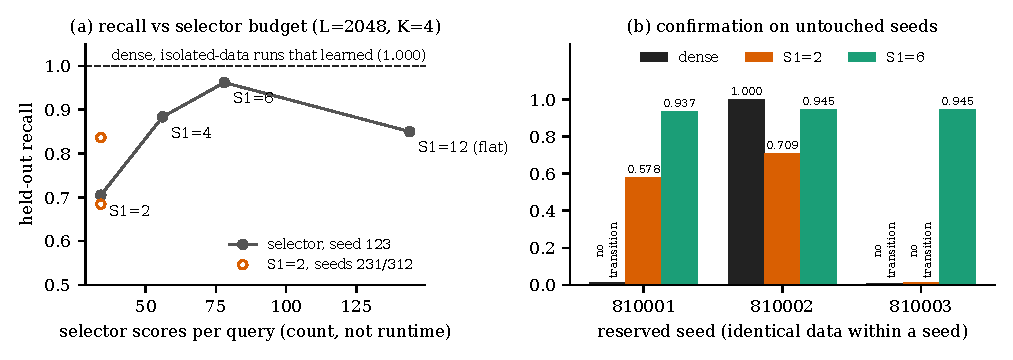
\includegraphics[width=\linewidth]{figures/fig1_budget.pdf}
\caption{\textbf{Recall rises from $S_1{=}2$ to $S_1{=}6$, but no setting matches dense attention where dense
learned.} (a) Held-out recall against selector scores per query on pilot seed 123 (filled), with $S_1{=}2$ on pilot
seeds 231 and 312 (open); $S_1{=}12$ is effectively flat selection. The dashed line marks dense recall on the
isolated-data runs where it transitioned. (b) Held-out recall on three untouched seeds; within a seed all models saw
identical data. ``No transition'' marks runs that never exceeded 0.30 validation recall within 60 epochs.
$L{=}2048$, $K{=}4$, 128 key--value pairs, M5 profile.}
\label{fig:budget}
\end{figure}

\section{Errors follow wrong choices, not failed reading}
\label{sec:selection}

To locate the loss we replayed the full held-out split (2{,}000 sequences, 256{,}000 queries) through all twelve
selector checkpoints of \S\ref{sec:budget}, using each run's own numerics and data, and recorded for each query
whether the retrieval layer selected the super-block and the fine block holding the queried key. Every replay first
had to reproduce its run's recorded held-out accuracy, loss and split fingerprint; all twelve did so exactly. The
analysis is descriptive and post hoc. Some finer probes below use earlier checkpoints from the M4 profile, labelled
as such (Appendix~\ref{app:runs}, Table~\ref{tab:selection_m4}).

\begin{table}[t]
\centering
\scriptsize
\begin{tabular}{llrrrrr}
\toprule
Setting & seed & recall & parent hit & key-block hit & recall $\mid$ hit & recall $\mid$ miss \\
\midrule
$S_1{=}2$ & 123 & 0.705 & 0.859 & 0.463 & 0.986 & 0.463 \\
$S_1{=}2$ & 231 & 0.684 & 0.861 & 0.627 & 0.999 & 0.155 \\
$S_1{=}2$ & 312 & 0.836 & 0.955 & 0.565 & 0.990 & 0.637 \\
$S_1{=}2$ & 810001 & 0.578 & 0.869 & 0.570 & 0.978 & 0.048 \\
$S_1{=}2$ & 810002 & 0.709 & 0.864 & 0.526 & 0.997 & 0.389 \\
$S_1{=}2$ & 810003$^\dagger$ & 0.011 & 0.809 & 0.383 & 0.022 & 0.005 \\
$S_1{=}4$ & 123 & 0.884 & 1.000 & 0.727 & 0.998 & 0.578 \\
$S_1{=}6$ & 123 & 0.962 & 1.000 & 0.962 & 1.000 & 0.002 \\
$S_1{=}6$ & 810001 & 0.937 & 1.000 & 0.933 & 1.000 & 0.060 \\
$S_1{=}6$ & 810002 & 0.945 & 1.000 & 0.845 & 1.000 & 0.644 \\
$S_1{=}6$ & 810003 & 0.945 & 0.996 & 0.748 & 1.000 & 0.781 \\
$S_1{=}12$ (flat) & 123 & 0.850 & 1.000 & 0.846 & 1.000 & 0.028 \\
\bottomrule
\end{tabular}
\caption{\textbf{Whenever the selector chose the key's block, the model answered correctly; from $S_1{=}4$ up it never
missed the key's super-block.} All twelve M5-profile selector runs, retrieval layer, full held-out split.
\emph{Parent hit}: the key's super-block was selected by at least one of the 4 heads; \emph{key-block hit}: the key's
block was among the $K{=}4$ blocks selected by at least one head. $^\dagger$Never transitioned.}
\label{tab:selection}
\end{table}

\paragraph{Reading is not the bottleneck at $K{=}4$.} For all eleven models that learned, recall was 0.978--1.000
whenever the retrieval layer selected the key's block (Table~\ref{tab:selection}); on the M4-profile checkpoints the
range was 0.993--1.000, and ablating the fine branch there dropped it to about 0.07, so correct answers come from
reading the selected tokens. The bottleneck is finding the block.

\paragraph{Why $S_1{=}6$ beats $S_1{=}2$: fewer wrong choices at both levels.} Although every key lies in super-blocks
0 and 1, the $S_1{=}2$ models missed the key's super-block on 4.5--14.1\% of queries (19.1\% for the run that never
learned). From $S_1{=}4$ upward these parent misses vanished (at most 0.4\%): with room beyond two super-blocks, the
right one was always kept. Fine-level choices improved too. Paired on the same seed, the key-block hit rate rose from
0.463 to 0.962 (seed 123), from 0.570 to 0.933 (810001) and from 0.526 to 0.845 (810002); parent misses fell from
0.13--0.14 to zero and fine-level misses from 0.30--0.40 to 0.04--0.16. Flat selection ($S_1{=}12$) never missed a
parent but chose the key's block less often than $S_1{=}6$ on the pilot seed (0.846 against 0.962), all of the
difference at the fine level, where it chooses among all past blocks rather than 66 candidates. That is one seed.

\paragraph{Recovering from a wrong choice is a seed-level property.} Recall after a key-block miss ranged from 0.002 to
0.781 across models, with no pattern by budget (Table~\ref{tab:selection}). On the M4-profile $S_1{=}2$ checkpoint
we examined this in detail: recall after a miss fell with the distance of the nearest selected block (0.76 at one
block away, 0.61 at two, 0.43 at three to eight), consistent with reading neighbouring blocks; but 13.9\% of its
queries had no selected block within eight blocks of the key and were still answered correctly 33\% of the time, so
some answers must come from another route, plausibly the coarse branch's attention over block summaries. We did not
isolate it.

\paragraph{The parent level can be solved by position.} In this MQAR layout every key lies in the first 256 tokens,
i.e.\ in super-blocks 0 and 1. A selector can therefore reach a high parent hit rate by preferring early
super-blocks instead of matching content: on the M4 profile, for queries at positions of 528 or more, 92.8\% of the
parent choices of one variant in \S\ref{sec:fixes} were exactly super-blocks $\{0, 1\}$. \textbf{Conclusions about
the parent budget $S_1$ may not transfer to tasks whose keys are spread across the context.} We return to this in
\S\ref{sec:limitations}.

\paragraph{The fine budget matters more than the parent budget, post hoc.} Changing the budgets of an M4-profile
checkpoint at inference only, on a 64-sequence subset (8{,}192 queries; hence 0.580 here against the full-split 0.594 in
Table~\ref{tab:selection_m4}), the key-block hit rate of the $S_1{=}2$ seed-123 model rose from 0.580 at $K{=}4$ to 0.769 at
$K{=}8$ and 0.884 at $K{=}16$, but only to 0.614 and 0.604 at $S_1{=}4$ and $S_1{=}6$ with $K{=}4$. Models trained at
$K{=}4$ would learn different scores at other budgets, so this is suggestive only; all trained results in this paper use
$K{=}4$.

\section{Two intuitive fixes made recall worse}
\label{sec:fixes}

Before M5 we tested whether the cheapest setting could be repaired without spending more selector work. Two causes
were plausible. First, the super-block scores feed only a hard top-$k$, so they receive no direct gradient from the
loss (the shared query and key projections still learn through the other branches). Second, super-block summaries
are mean-pooled, which may blur the single key a query needs. We pre-registered three variants at the same budget
($S_1{=}2$, $K{=}4$): a \emph{router gate} that adds a log-sigmoid of each selected super-block's score to the logits of its
child blocks in the coarse branch and of their tokens in the fine branch, giving the parent scores a gradient path
(the hard top-$k$ choices still use the ungated scores); \emph{max-pooled} super-block summaries; and both. All
four arms trained on identical data from identical initial weights (seed 123, M4 profile), and a fix counted as a
recovery only if it gained at least 0.10 held-out recall.

\begin{table}[t]
\centering
\small
\begin{tabular}{lrrrr}
\toprule
Arm ($S_1{=}2$, seed 123) & held-out recall & change & key-block hit & recall $\mid$ miss \\
\midrule
baseline & 0.803 & -- & 0.594 & 0.516 \\
router gate & 0.652 & $-0.151$ & 0.648 & 0.025 \\
max-pool summaries & 0.648 & $-0.155$ & 0.629 & 0.057 \\
both & 0.751 & $-0.052$ & 0.708 & 0.163 \\
\bottomrule
\end{tabular}
\caption{\textbf{Each repair found the key block more often yet recalled less; recall after a miss nearly
vanished.} One seed, identical data and initialisation across arms, M4 profile, $S_1{=}2$, $K{=}4$.}
\label{tab:fixes}
\end{table}

\textbf{No variant recovered recall; all three lowered it} (Table~\ref{tab:fixes}). The selection diagnostic shows
why the numbers moved. Each fix raised the key-block hit rate (0.594 to 0.629--0.708) but nearly removed the
correct answers after a miss: recall on a miss fell from 0.516 to 0.025--0.163. This accounts for the lower
recall arithmetically; it is not a causal explanation. Two further observations limit the reading. The router gate
and max-pooling each \emph{lowered} the parent hit rate (0.873 and 0.830 against 0.888), and the combined arm's
near-perfect parent hit (0.999) is the positional shortcut of Section~\ref{sec:selection}. Finally, this is one seed, and
two baseline seeds already differed by 0.105 in key-block hit rate. We conclude only that these two remedies failed
this screen, not that gradient-free routing or summary dilution are unimportant.

\section{Dense attention trains unreliably on this recipe}
\label{sec:dense}

The dense baseline was the least reliable model in the study. On the isolated data, dense attention transitioned
within 60 epochs on two of the four seeds we tried (two of seven runs, counting reruns in float32); the $S_1{=}6$ selector
transitioned on all four seeds, and the selector as a whole in 11 of 12 M5-profile runs (Figure~\ref{fig:dense}). When dense did transition it reached 1.000, so this is a finding about training
reliability within a fixed budget, not about recall capacity.

\begin{figure}[t]
\centering
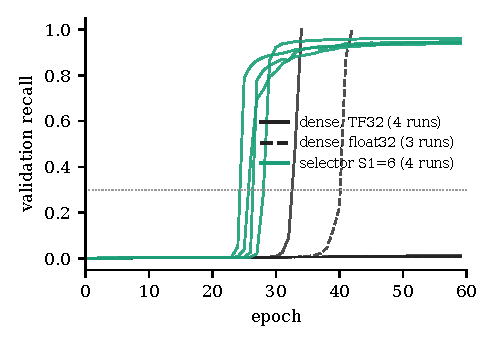
\includegraphics[width=0.6\linewidth]{figures/fig2_training.pdf}
\caption{\textbf{On identical data, the sparse selector learned every time and dense attention mostly did not.}
Validation recall per epoch for the seven dense runs (solid: TF32; dashed: float32) and four $S_1{=}6$ runs on
seeds 123 and 810001--810003, isolated data. The dotted line is the 0.30 transition threshold. One float32 dense run
(seed 810001) was stopped after 55 of 60 epochs.}
\label{fig:dense}
\end{figure}

\paragraph{Neither numerics nor the data generator alone explains it.} M5 changed two things at once relative to
M4: TF32 matrix multiplication and the isolated data generator. On seed 123 we separated them
(Table~\ref{tab:densecheck}). Dense learned under TF32 with the legacy data (transition at epoch 26, 0.987) and in
float32 with the isolated data (epoch 41, 1.000). With one run per cell, this is consistent with the isolated data delaying
the transition, and with ordinary seed-level chance; the pre-registered reading allowed both. We then reran dense in float32 on the two reserved seeds where it had failed. Neither
transitioned: seed 810003 finished at 0.0069 held-out recall, and seed 810001 was stopped at epoch 55 of 60 with best
validation recall 0.0068, so it has no held-out score.

\begin{table}[t]
\centering
\small
\begin{tabular}{llrr}
\toprule
Numerics & Data generator & held-out recall & transition epoch \\
\midrule
float32 & legacy (M4) & 0.992 & 28 \\
TF32 & legacy & 0.987 & 26 \\
float32 & isolated & 1.000 & 41 \\
TF32 & isolated (M5) & 0.010 & never \\
\bottomrule
\end{tabular}
\caption{\textbf{Dense learned under each change alone, but late on the isolated data.} Dense attention, seed 123,
one run per row. Row 1 is the M4 follow-up (earlier code revision); rows 2 and 3 were run to separate the two
changes made between M4 and M5.}
\label{tab:densecheck}
\end{table}

\paragraph{What this means for the comparison.} One explanation is that dense attention's phase transition on this
task arrives at a time that varies widely with the data draw and the numerics, and that our 60-epoch budget cuts off
the late cases. Two observations caution against reading this as only a matter of time. The cosine schedule brings
the learning rate close to zero by epoch 60, so a longer ceiling would also change the schedule. And in every failed
dense run validation loss reached its minimum between epochs 16 and 21 and then rose; in the float32 reruns training
loss kept falling, to about 7.2 against about 8.1 on validation, a pattern consistent with memorising the 20{,}000
training sequences. We did not test either explanation, and we did not change the recipe after seeing the data. The comparison is also not perfectly matched: the dense baseline applies dropout 0.1 inside
attention and the selector does not, and the two mixers differ in parameters (the selector adds branch gates).
Either difference could affect when the transition arrives. Its consequence is concrete: on seeds 810001 and 810003 the selector learned (0.937 and 0.945 at
$S_1{=}6$) where full attention, on identical data and recipe, did not. It also means the study has a single valid
dense-versus-selector pair (seed 810002), which is why we report its gaps as observations rather than estimates.

\section{Related work}
\label{sec:related}

\paragraph{Sparse and hierarchical attention.} Fixed sparsity patterns~\cite{child2019sparse,beltagy2020longformer,
zaheer2020bigbird} and content-based routing~\cite{kitaev2020reformer,roy2021routing} reduce attention's quadratic
cost; Routing Transformer already reached $O(n^{1.5})$ with content-based clustering~\cite{roy2021routing}.
Block-level selection is now common: Quest chooses key pages per query at inference time~\cite{tang2024quest}, MoBA
routes each query to a few trained blocks~\cite{lu2025moba}, Landmark Attention and InfLLM retrieve blocks through
representative tokens~\cite{mohtashami2023landmark,xiao2024infllm}, DeepSeek Sparse Attention selects tokens with a
lightweight learned indexer~\cite{deepseek2025v32}, and NSA~\cite{yuan2025nsa} combines compressed, selected and windowed
branches with trainable sparsity; our selector inherits NSA's three-branch layout. Hierarchical selection is well established: HiP prunes a tree of key blocks without
training~\cite{lee2025hip}, HISA filters pooled blocks before refining to tokens~\cite{xu2026hisa}, gist-token methods
learn chunk summaries and recursive summary hierarchies~\cite{mao2026gist}, and HiLS trains chunk-level retrieval scores
through the language-model loss~\cite{hu2026hils}. Several of these papers vary their selection budget and report
retrieval-sensitive benchmarks. Our
selector is a simpler member of this family, and we claim no algorithmic novelty. HiLS is closest in spirit; it
measures retrieval in small models under matched sparse budgets on RULER. We differ in scale and in protocol: one
synthetic task, but a dense model on byte-identical splits for every comparison, reserved confirmation seeds, and
every failed run reported. The Sparse Frontier studies sparsity--accuracy trade-offs of training-free methods in
large pretrained models across tasks and lengths~\cite{nawrot2025sparsefrontier}; our setting is the opposite end:
models trained from scratch with the selector, at toy scale. Two recent methods train selection end to end: SAS injects
the selector's continuous scores into attention logits so the language-modelling loss trains the ranking, and
compares gate forms~\cite{li2026sas}; FreeSolo pairs a sliding window with a learned long-range cell selector and
reports zero-shot length extrapolation~\cite{shi2026freesolo}. Our failed router gate (Section~\ref{sec:fixes}) is one
implementation on one task and does not test those designs.

\paragraph{Recall in efficient sequence models.} Zoology introduced MQAR and showed that most of the quality gap
between attention and gated-convolution models comes from associative recall~\cite{arora2024zoology}. Later work
traced a trade-off between recall and recurrent state size in linear attention~\cite{arora2024based} and proved and measured that fixed-state
models copy worse than transformers~\cite{jelassi2024repeat}; MQAR results for recurrent models are also sensitive to the
learning rate, which can make capacity conclusions from untuned runs misleading~\cite{okpekpe2025revisiting}. Long-context evaluations show that models use
information unevenly across their inputs~\cite{liu2024lost}. These studies compare architectures; we hold the
architecture fixed and vary how much of the context a sparse selector may consider.

\paragraph{Efficiency claims and their evaluation.} Kernel-level work such as FlashAttention reports speed with its
hardware, lengths and baselines stated~\cite{dao2022flashattention}. Some recent commercial reports pair large
long-context speed-ups with benchmark scores but without a dense model trained under matched
settings~\cite{subq2026,appen2026}. We do not evaluate those systems, whose mechanisms are not public. We use identical data to remove one source of confounding;
the remaining mixer and optimisation differences (Section~\ref{sec:dense}) still prevent attributing the whole
dense--selector gap to sparsity alone, and within-model controls are an equally valid design.

\section{Limitations}
\label{sec:limitations}

\paragraph{A positional shortcut in the task.} Zoology's MQAR places every key in the first 256 tokens, so the
coarse level can be solved by preferring early super-blocks (\S\ref{sec:selection}). Conclusions about $S_1$ may not
transfer to tasks whose keys are spread across the context. We built a variant with keys placed anywhere, but dense
attention did not learn it under this recipe (recall 0.0002--0.0044, near chance, across four variants), so it could not serve
as a test. A learnable shortcut-free task is the most important next step.

\paragraph{One valid dense comparison.} Dense attention transitioned on only one of the three reserved seeds, so the
gaps of 0.291 and 0.055 rest on a single pair. They are observations, not estimates, and we make no claim of
statistical significance. The dense column also mixes numerics: the valid pair is TF32, while the float32 reruns are
diagnostics.

\paragraph{A selected operating point.} $S_1{=}6$ was chosen after the pilot because it scored highest there. The
reserved seeds confirm that point only; $S_1{=}4$ and $S_1{=}12$ were not run on them.

\paragraph{Training ceiling and a stopped run.} A non-transition means only that validation recall did not exceed
0.30 within 60 epochs of a cosine schedule that ends near zero learning rate; a longer or different schedule could
change any such run. The recipe was not tuned for dense attention under the M5 profile. One float32 dense
run (seed 810001) was stopped by us after 55 of 60 epochs with validation recall at 0.0068, and has no held-out score.

\paragraph{Scale and scope.} Models have 2 layers and width 128; there is one task and one length (2048). We make no
claim about real text, longer contexts or larger models. At length 4096 even dense attention failed under this
recipe, and longer lengths fall outside the task's vocabulary constraint.

\paragraph{Mixers are matched in width, not in everything.} Dense attention uses dropout 0.1 and the selector
none; the selector has extra gate parameters. Either could contribute to the difference in training reliability.

\paragraph{The budget knob is not a pure intervention.} Raising $S_1$ also enlarges the set of blocks the fine level
chooses from, and on this task the parent level can be solved by position, so the budget curve mainly reflects how
reliably the fine choice is learned (\S\ref{sec:budget}). Flat block selection was run only as $S_1{=}12$, on one seed
per profile, so whether the hierarchy helps or costs recall is not settled. The fine budget $K$ was fixed at 4; a
post-hoc probe suggests it matters more than $S_1$ (\S\ref{sec:selection}).

\paragraph{No speed claim.} Selector scores per query is a count, not runtime. Without a fused kernel our selector
was slower than dense attention at every budget (Table~\ref{tab:cost}).

\paragraph{Mechanism evidence is post hoc.} The selection diagnostic (\S\ref{sec:selection}) replays trained models
and describes their choices; it does not intervene on them. The repair screen (\S\ref{sec:fixes}), the distance
analysis and the budget probe use one M4-profile checkpoint per arm, and their explanations account for the numbers
arithmetically rather than causally.

\section{Conclusion}
\label{sec:conclusion}

On MQAR at length 2048 with a fixed fine budget, a two-level block selector recalled more as it kept more
super-blocks, up to a point: on identical data, keeping six beat keeping two on all four seeds, and keeping all twelve
(effectively flat selection) did worse on the one seed where both were run. Where dense attention learned, it beat
both settings run on that seed, by 0.291 at the cheapest and 0.055 at six super-blocks, so none met our pre-registered bar of 0.02.
Because this task lets the coarse level be solved by position, the curve speaks to how reliably the selector learns to
choose, not to information lost by pruning. Replaying the trained models, errors followed wrong block choices rather than failed
reading; the cheapest setting kept missing the right super-block despite the shortcut, and two intuitive repairs made
recall worse. Dense attention itself learned on only two of four seeds
within our training budget. These results come from one synthetic task with a positional shortcut, small models and few
seeds. We hope the protocol---matched data, reserved seeds, and every failure reported---is useful to others
measuring what sparse attention gives up.


\bibliographystyle{plainnat}
\bibliography{refs}

\appendix
\section{All runs}
\label{app:runs}

Table~\ref{tab:allruns} lists every run on the M5 profile together with the dense diagnostics of
Section~\ref{sec:dense}; it is generated from the committed run records by \texttt{paper/make\_tables.py}.
Table~\ref{tab:m4runs} lists every run on the earlier M4 profile, whose checkpoints are analysed in
Sections~\ref{sec:selection} and~\ref{sec:fixes}. The two profiles are never pooled. Not listed: smoke tests, and one M4 launch cancelled at about epoch 13 when its
launching machine lost its session, which the protocol classes as incomplete.

\begin{table}[h]
\centering
\scriptsize
\begin{tabular}{lrllrrrrr}
\toprule
Model & seed & numerics & data & round & held-out & best val. (epoch) & transition & epochs \\
\midrule
$S_1{=}2$ & 123 & TF32 & isolated & M5 & 0.705 & 0.704 (53) & 41 & 60 \\
dense & 123 & TF32 & isolated & M5 & 0.010 & 0.010 (55) & never & 60 \\
$S_1{=}2$ & 231 & TF32 & isolated & M5 & 0.684 & 0.685 (46) & 40 & 60 \\
$S_1{=}2$ & 312 & TF32 & isolated & M5 & 0.836 & 0.837 (46) & 35 & 60 \\
$S_1{=}12$ & 123 & TF32 & isolated & M5 & 0.850 & 0.850 (37) & 26 & 60 \\
$S_1{=}4$ & 123 & TF32 & isolated & M5 & 0.884 & 0.885 (59) & 34 & 60 \\
$S_1{=}6$ & 123 & TF32 & isolated & M5 & 0.962 & 0.962 (58) & 29 & 60 \\
dense & 810001 & TF32 & isolated & M5 & 0.012 & 0.012 (58) & never & 60 \\
$S_1{=}2$ & 810001 & TF32 & isolated & M5 & 0.578 & 0.578 (59) & 49 & 60 \\
dense & 810002 & TF32 & isolated & M5 & 1.000 & 1.000 (34) & 33 & 35 \\
$S_1{=}2$ & 810002 & TF32 & isolated & M5 & 0.709 & 0.709 (42) & 39 & 60 \\
dense & 810003 & TF32 & isolated & M5 & 0.006 & 0.007 (53) & never & 60 \\
$S_1{=}2$ & 810003 & TF32 & isolated & M5 & 0.011 & 0.011 (58) & never & 60 \\
$S_1{=}6$ & 810001 & TF32 & isolated & 2c & 0.937 & 0.937 (56) & 25 & 60 \\
$S_1{=}6$ & 810002 & TF32 & isolated & 2c & 0.945 & 0.946 (56) & 27 & 60 \\
$S_1{=}6$ & 810003 & TF32 & isolated & 2c & 0.945 & 0.944 (58) & 26 & 60 \\
dense & 123 & TF32 & legacy & check & 0.987 & 0.987 (27) & 26 & 28 \\
dense & 123 & float32 & isolated & check & 1.000 & 1.000 (42) & 41 & 43 \\
dense & 810001 & float32 & isolated & 2e & --$^\ddagger$ & 0.007 (54) & never & 55 \\
dense & 810003 & float32 & isolated & 2f & 0.007 & 0.007 (57) & never & 60 \\
\bottomrule
\end{tabular}
\caption{\textbf{Every run on the M5 profile and its diagnostics, including all non-transitions.} Epochs are zero-based; early stopping at validation recall above 0.98 ends some runs before 60 epochs. $^\ddagger$Stopped by us after 55 of 60 epochs; no held-out score.}
\label{tab:allruns}
\end{table}


\begin{table}[h]
\centering
\small
\begin{tabular}{lrrrrr}
\toprule
Model (seed) & recall & parent hit & key-block hit & recall $\mid$ hit & recall $\mid$ miss \\
\midrule
$S_1{=}2$ (123) & 0.803 & 0.888 & 0.594 & 0.999 & 0.516 \\
$S_1{=}2$ (312) & 0.715 & 0.815 & 0.489 & 0.997 & 0.446 \\
$S_1{=}12$ (123) & 0.920 & 1.000 & 0.729 & 1.000 & 0.705 \\
$S_1{=}2$ (231), never learned & 0.008 & 0.707 & 0.274 & 0.014 & 0.005 \\
\bottomrule
\end{tabular}
\caption{\textbf{Selection diagnostic on the earlier M4-profile checkpoints.} Retrieval layer, full held-out split. \emph{Parent hit}: the key's super-block was selected by at least one of the 4 heads;
\emph{key-block hit}: the key's fine block was among the $K{=}4$ blocks selected by at least one head. Recall conditioned on a key-block hit
was 0.997--1.000 for every model here that learned.}
\label{tab:selection_m4}
\end{table}

\begin{table}[h]
\centering
\scriptsize
\begin{tabular}{llrrrr}
\toprule
Experiment & Model & seed & held-out & best val.\ (epoch) & transition \\
\midrule
repair screen & $S_1{=}2$ baseline & 123 & 0.803 & 0.803 (45) & 35 \\
repair screen & $S_1{=}2$ router gate & 123 & 0.652 & 0.651 (40) & 39 \\
repair screen & $S_1{=}2$ max-pool & 123 & 0.648 & 0.648 (46) & 42 \\
repair screen & $S_1{=}2$ both & 123 & 0.751 & 0.752 (28) & 28 \\
follow-up & dense & 123 & 0.992 & 0.992 (29) & 28 \\
follow-up & $S_1{=}12$ & 123 & 0.920 & 0.920 (57) & 25 \\
follow-up & $S_1{=}2$ & 312 & 0.715 & 0.715 (58) & 40 \\
follow-up & $S_1{=}2$ & 231 & 0.008 & 0.007 (54) & never \\
\bottomrule
\end{tabular}
\caption{\textbf{Every run on the M4 profile} (float32, legacy data). All four repair-screen arms trained on
identical data from identical initial weights. Each run used its own data; seeds 231 and 312 are not paired with
seed 123.}
\label{tab:m4runs}
\end{table}

\section{Compute}
\label{app:compute}

Every run used a single NVIDIA L40S GPU, on AWS (\texttt{g6e.xlarge}) or Modal, one run per GPU at a time. M5-profile
runs took 0.9--4.6 hours each. Software versions differed slightly between machines (PyTorch 2.14.0 or 2.14.1 with
CUDA 13.0; Python 3.11 or 3.13); each run's manifest records its environment. The experiments in this paper used
roughly \$150 of cloud GPU time; the M5 selection diagnostic (inference only, twelve L40S containers on Modal) cost
under \$2.

\section{Earlier exploratory results}
\label{app:history}

Before the protocol of Section~\ref{sec:setup} was fixed, the project ran exploratory experiments that report
\emph{validation} recall from single runs with differing recipes. We list them for context only; none enters the
results above. At length 128, attention reached 0.998 against 0.097 for a gated convolution, reproducing Zoology's
recall gap. At length 2048, an unpruned selector ($S_1{=}12$) and dense attention both reached about 0.99 validation
recall, while two recurrent baselines reached 0.558 and 0.193 (the first with a different learning rate). At length
4096 every model, including dense attention, failed to learn. An early reading of these runs, that block sparsity
alone caused the recall loss at length 2048, was retracted once budget sweeps showed recall rising with the budget. These runs are not part of the public release.

\section{Reproduction}
\label{app:repro}

Code, frozen protocols, per-run manifests (seeds, SHA-256 split hashes, environment, code commit), per-epoch
metrics, training logs, the selection-diagnostic scripts (\texttt{experiments/diagnose\_routing.py},
\texttt{experiments/modal\_diagnose\_m5.py}) and their outputs, and the scripts that regenerate the figures
and the appendix tables are at
\url{https://github.com/eumnesia-labs/sparse-attention-recall} (release v1.2). Figures: \texttt{python3 paper/figures/make\_figures.py};
appendix table: \texttt{python3 paper/make\_tables.py}; each results folder's \texttt{summarize*.py} regenerates its
summary from raw records. The M5 runs used a cloud version of the training harness that also contains unrelated,
unpublished work and is not released. The release instead provides a portable runner with the same recipe
(\texttt{--task mqar --precision tf32}), and \texttt{experiments/reproduce\_m5.py} turns any stored manifest into a
local command without the cloud steps. The portable runner has not been checked for numerical equivalence with the
original runs; hardware, library versions and nondeterminism can change outcomes. Training a model requires one GPU.
Model checkpoints are not released.


\end{document}
